\documentclass[stu,12pt]{apa7}
  \usepackage{times}               % Times New Roman Font Face
  \usepackage[american]{babel}     % Localization
  \usepackage[utf8]{inputenc}      % Input Encoding
  \usepackage{hyperref}            % Hyperlinks
  \usepackage{enumitem}            % Additional Enumeration Environment Settings
  \usepackage{geometry}            % Page Layout
  \usepackage{soul}                % Text Highlighting
  \usepackage{graphicx}            % Images
  \usepackage{csquotes}            % Quoting Environment
  \usepackage{bookmark}            % Required by `csquotes'
  \usepackage{mdframed}            % Colorful Tex-Box Environment
  \usepackage[toc]{appendix}       % Appendix
  \usepackage{fancyhdr}            % Headings and Footers
  \usepackage[%
    style=apa,%
    sortcites=true,%
    sorting=nyt%
  ]{biblatex}
  \usepackage{xcolor}

  % Bibliography Setup
  %% Language Mappings
  \DeclareLanguageMapping{english}{english-apa}
  \DeclareLanguageMapping{american}{american-apa}
  %% Bibliography File Path
  \addbibresource{main.bib}
  %% Categories for Specified Bibliography Items
  %%% Category for sources not referenced in-text
  \DeclareBibliographyCategory{consulted}
  \addtocategory{consulted}{noauthor_business_nodate}
  \addtocategory{consulted}{noauthor_college_nodate}
  \addtocategory{consulted}{apatow_this_2012}
  \addtocategory{consulted}{cuddy_your_2012}
  \addtocategory{consulted}{anonymous_changing_1999}
  \addtocategory{consulted}{paturel_talk_2012}
  \addtocategory{consulted}{safdar_variations_2009}

  % Images
  \graphicspath{ {./res/img} }

  % Hyperlink Setup
  \hypersetup{
    colorlinks = true,
    urlcolor = blue,
    linkcolor = blue,
    citecolor = blue
  }

  % Page and Text Layout
  \geometry{%
    a4paper,%
    top=1in,%
    bottom=1in,%
    left=1in,%
    right=1in%
  }
  \setlength{\headheight}{15pt}

  % Header
  \lhead{COM125CG1-M4D1}

  % Title Page
  \title{%
    M4D1: Communicating Without Words
  }
  \shorttitle{Module 4 Discussion 1}
  \author{Ashton Hellwig}
  \authorsaffiliations{Department of Mathematics, Front Range Community College}
  \course{COM125: Interpersonal Communication}
  \professor{Richard Thomas}
  \duedate{November 28, 2020 23:59:59 MDT}
  \date{\today}
  \abstract{%
    \textbf{Overview}\\%
    Just like countries have different languages, our nonverbal communication
      may not equate to the same meaning. For example, the thumbs up gesture
      means ``good job'' in the United States. But in the Middle East, it’s
      the equivalent of an insult! That’s a significant difference in meaning
      that could lead to huge misunderstandings.\\%

    For this discussion, you will research nonverbal communication in another
      country's culture (outside of the United States) and compare and
      contrast nonverbal communication in the country you selected with your
      home country's culture.\\%

    As we saw in the movie clip appearing within the topic titled, ``The
      Theme'' and in the TED Talk titled, ``The Importance of Listening'', our
      body language often communicates messages in addition to our verbal
      communication. Reflect for a few moments on how your body language
      messages might be received by people from a different culture who do not
      understand the intended meaning of your nonverbal communication.\\%

    You should spend approximately 4 hours on this assignment.\\%
    \vspace{14px}
    {%
      \centering%
      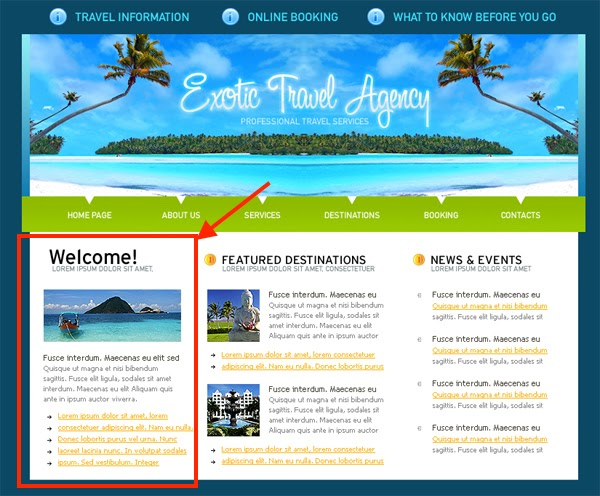
\includegraphics[%
        scale=0.6%
      ]{instructions_travelagency.jpg}%
      \par%
    }
  }

\begin{document}
  % Title Page
  \maketitle

  % Initial Post
  \section{Initial Post}
    \subsection*{Instructions}
      \begin{enumerate}
        \item Be sure you have completed your readings and explored all the
          materials, including videos, in the Exploration page accessible
          within the ``Read/View'' topic of Module 4 Content.

        \item Research the culture of another country with which you are
          either familiar or unfamiliar.

        \item In your research, focus on nonverbal communication.
          Specifically, consider gestures, facial expressions, and proximity
          (i.e., how close people stand to each other). In addition, research
          whether nonverbal communication is different between genders in the
          culture you have selected.

        \item Include and answer the following questions in your main post:
          \begin{itemize}
            \item In your own words, define language and nonverbal
              communication. How is the nonverbal communication of the culture
              you researched different from nonverbal communication in your
              home country's culture? How is nonverbal communication similar
              or the same?

            \item What are the differences in nonverbal communication between
              genders in the culture you researched? If there are no
              differences, why do you feel nonverbal communication between
              genders is the same?

            \item What was the most surprising difference between your home
              country's culture and the country's culture you chose to from
              this Discussion assignment?

            \item Write a sidebar (3--4 sentences) that could be highlighted
              on the Travel Channel's website for readers traveling to the
              country you researched on how they should greet a stranger from
              the other culture. Include at least three tips. Consider
              questions such as, should they bow? Wave? Offer their hand to
              shake? Would they greet a man differently than a woman? How
              close should they stand? Should they smile?
          \end{itemize}
      \end{enumerate}


    \newpage
    \subsection{Language and Non-Verbal Communication}
      \subsubsection{Defining Language}
        Language, at its easiest definition, is a collection of the syntax
          rules and vocabulary with which we speak verbally to one-another.
      \subsubsection{Defining Non-verbal communication}
        Non-verbal communication is when we use any other action other than
          speaking words to generate meaning or express an idea
          \parencite[pp. 224]{noauthor_communication_2013}.

    \subsection{The People of Japan's Communication}
      \subsubsection{How Japan Communicates Non-Verbally}
        Placeholder.
      \subsubsection{Comparing Non-Verbal Communication in Japan and the U.S.A.}
        The non-verbal communication cues utilized by Americans and Japanese
          residents is not \textit{completely} divergent. For example, with
          facial expressions, us two cultures tend to share similar
          representations of negative emotions
          \parencite[pp. 75]{lafrance_cultural_1978}. There are still some
          differences in in how we express many other emotions, including
          negative ones. In Japan, it is noted that when someone is annoyed
          they may represent this with a ``Pan Am Smile'' (the
          \textit{opposite} of a genuine smile of happiness --- called the
          ``Duchenne Smile''). It is said that this is for the annoyed listener
          to display the fortitude of their inner strength and control
          \parencite[pp. 76]{lafrance_cultural_1978}.
      \subsubsection{Gender's Role In Non-Verbal Communication in Japan}
        While Japan does have many different masculine and feminine pronouns,
          the focus is not necessarily \emph{entirely} on gender. The primary
          hierarchy in Japan is instead mostly concerned with \textbf{senority}.
          This is not to say just within the business world, in which it is
          prevelant, but also in the grammar rules engrained in the Japanese
          language. The concept ``Senpai and Kohai'' is the
          ``Senior and Junior'' relationship which, while most prevelant in
          schools, is seen \textit{everywhere} around Japan. It is essentially
          the idea of respecting our elders taken to such an extreme that is
          now a permanent part of Japanese culture, as it has been for centuries
          \parencite[pp. 253]{potts_japanese_nodate}.
      \subsubsection{Conclusion}
        \paragraph{The Most Surprising Differences Between Japan and the U.S.A.}
          I believe on the most surprising differences between the cultures of
            the United States of America and that of Japan would have to be
            the level of hierarchy we notice in Japan. Working in the Marijuana
            industry here in Colroado, we see the opposite of what is standard
            in Japan due to how \textit{young} our industry is. It is not
            all that uncommon to see the owner or general manager of a retail
            location in this industry \textbf{incredibly young}, usually in
            their late 20s and early 30s. Many times, for the companies I have
            worked for, I have coworkers and peers that are twice my age while
            our manager will be in their mid twenties. In Japan, they even have
            a system in use at some companies where promotions and pay raises
            are given out ``based on one's proximity to retirement''
            \parencite{lafrance_cultural_1978}.

    \subsection{How to Communicate whilst Traveling to Japan}
      \begin{enumerate}
        \item Ensure you know your ``role'' in comparison to the person you
          are speaking with. The easiest way to do this is to ask for a
          business card or hear how your peers address that person.
        \item Bowing is an incredibly important practice in use in Japan,
          especially for formal meeting scenarios (school, work, loved one's
          parents).
        \item In the United States we tend to think of the most senior/important
          person speaking first, but in Japan, the most senior and/or most
          important person is who tends to speak last in a group.
      \end{enumerate}


  % Replies
  % %! TEX root=../main.tex

\section{Responses}
  \subsection{Response 1}
    \begin{quotation}
      Listening is something that comes easier to me than talking.
        As I indicated by my goals, one of which is to be less concise, I do not
        often just volunteer information about myself.  I prefer to listen to
        what others have been thinking about or learn more about them. I can
        relate to Erin because I would probably be wondering why I did not get
        the bonus that they had talked about, although instead of making a fuss
        about it I would probably have just checked out of the situation.
        Overall, the way Ed started the conversation, despite the fact he was
        trying to surprise her, would have caused anyone to be a bit upset.
        I do not really think that gender had anything to do with this situation
        and the reactions they had. It seems to me that this would have been
        more influenced by personality, not gender.

      I believe that we can define listening as processing information or
        emotions from others.  One article I read when studying effective and
        not effective listening skills, which talks about things effective
        listeners do states, “These behaviors include responses such as
        ``uh huh'' and ``hmmm,'' as well as other nonverbal behaviors including
        nodding, smiling, and adjusting one's posture. Other active listening
        behaviors include asking questions, making eye contact, and not
        interrupting the speaker” (Fedesco, 2015).  Asking questions can help
        you to not only better remember information, but also better understand
        it. That article goes on to say that the more you use those behaviors
        indicates how invested you are in a certain conversation. Another
        article I read makes this claim that being a good listening can offer,
        ``A greater number of friends and social networks, improved self-esteem
        and confidence, higher grades at school and in academic work, and even
        better health and general well-being'' (Listening Skills). This means
        that being a good listener can provide a large number of benefits. Being
        a good or bad listener would definitely affect your grades in school.

      As I tried to find a difference between male and female in terms of
        listening, I did not find anything that indicated one listens better
        than the other.  I read an article which states, “Despite activating
        different activity centers within the brain, genders perform equally on
        measures of cognitive function. This means that although we listen and
        assimilate information differently, the difference does not appear to
        affect cognition or our ability to listen” (McCormick,2018). Therefore,
        our brains may function in a different way, but that does not indicate
        that either men or women listen better simply based on their gender.
        I would say my research aligns pretty well with how I communicate, with
        exception to the occasionally accidental interruption.  Therefore, I
        would still classify myself as a good listener.  I often ask questions,
        make eye contact, and am sympathetic to the person speaking.

      Effective Listeners Top 5 List:
      \begin{enumerate}
        \item Asking questions
        \item Making eye contact
        \item Not interrupting
        \item Smiling
        \item Being polite
      \end{enumerate}

      Ineffective Listeners Top 5 List
      \begin{enumerate}
        \item Interrupting
        \item Looking away
        \item Crossing their arms
        \item Not reacting with smiles or frowns (not sympathetic)
        \item Often changing the subject
      \end{enumerate}
    \end{quotation}

    \paragraph{This is a response to Thora Smith on Post ID 43465667}
      Placeholder.

  % %! TEX root=../main.tex

\subsection{Response 2}
  \begin{quotation}
    Placeholder.
  \end{quotation}

  \paragraph{This is a response to FIRST LAST on Post ID 00000000}
    Placeholder.



  % Bibliography
  %% Works Cited
  \newpage
  \printbibliography[%
    title={References},%
    heading={bibintoc},%
    notcategory={consulted}%
  ]

  %% Works Consulted
  \newpage
  \nocite{*}
  \printbibliography[%
    title={Additional References},%
    heading={bibintoc},%
    category={consulted}%
  ]
\end{document}
